%\documentclass[11pt]{scrartcl}
\documentclass[11pt, twoside, a4paper, BCOR8mm, DIV12, bibtotoc,idxtotoc]{scrbook}
\usepackage{german}
\usepackage{typearea}
\usepackage[utf8]{inputenc}
\usepackage{longtable}
\usepackage{hyperref}
\usepackage{graphicx}

% Zusaetzliche Picture-Umgebungen (z.B. shadowenv)
\usepackage{picins}

% Header anpassbar
\usepackage{fancyhdr}

% Headings umdefinieren
\pagestyle{fancy}
\fancyhf{}
\fancyhead[RO]{\nouppercase{\rightmark}}
\fancyhead[LE]{\nouppercase{\leftmark}}
\fancyfoot[RO, LE]{\thepage}

%\addtolength{\headwidth}{\marginparsep}
%\addtolength{\headwidth}{\marginparwidth}
\addtolength{\headwidth}{1cm}

\parindent0.0mm
\parskip0.3cm    
\typearea{13}

\begin{document}

\frontmatter

\begin{titlepage}

\begin{center}
\rule[-.1in]{16cm}{1mm}\\[3mm]
{\fontfamily{cmss}\fontseries{bx}\fontshape{n}\fontsize{20}{20pt}\selectfont
  www.openbib.org $\bullet$ OpenBib Rechercheportal}\\[-2mm]
\rule[-.1in]{16cm}{1mm}

\vspace{5cm}

  \textbf{\fontfamily{cmss}\fontseries{bx}\fontshape{n}\fontsize{30}{30pt}\selectfont OpenBib Recherche-Portal\\[3mm] Technische Dokumentation}

  \vspace{2cm}

  Oliver Flimm \texttt{<flimm@openbib.de>}\\
  Stand: 15.6.2006

  \vspace{8cm}

\rule[-.1in]{16cm}{1mm}\\[3mm]
{\fontfamily{cmss}\fontseries{bx}\fontshape{n}\fontsize{20}{20pt}\selectfont
  www.openbib.org $\bullet$ OpenBib Rechercheportal}\\[-2mm]
\rule[-.1in]{16cm}{1mm}

\end{center}

\end{titlepage}

%\thispagestyle{empty}

%\begin{verbatim}


%Copyright (c) 2004-2006 Oliver Flimm <flimm@openbib.org>

%Es wird die Erlaubnis gegeben dieses Dokument zu kopieren, verteilen 
%und/oder zu veraendern unter den Bedingungen der GNU Free
%Documentation License, Version 1.1 oder einer spaeteren, von der Free 
%Software Foundation veroeffentlichten Version; mit den
%Unveraenderlichen Abschnitten DEREN TITEL AUFGEZAEHLT sind, mit den 
%Vorderseitentexten die AUFGEZAEHLT sind, und mit den Rueckseitentexten
%die AUFGEZAEHLT sind. Eine Kopie dieser Lizenz ist in dem Abschnitt 
%enthalten, der mit "GNU Free Documentation License"
%\end{verbatim}

\tableofcontents

\mainmatter


\chapter{Generelle Features}
Um einen schnellen Überblick von den Fähigkeiten und Möglichkeiten 
des OpenBib Recherche-Portals in der Version 2.0 und höher zu
bekommen sowie eine Entscheidungshilfe für einen möglichen Einsatz
zu geben, beginnt dieses technische Handbuch mit einer Aufzählung der
generellen Features des Portals.

\section{OpenBib ist OpenSource}
Bei dem OpenBib Recherche-Portal handelt es sich um
OpenSource-Software. Damit ist eine maximale Freiheit bei der
Anpassung an die individuellen Anforderungen gewährleistet.
Darüber hinaus ist die Eintrittsschwelle in die Änderung oder
Erweiterung des Portals durch die Ver\-wen\-dung des DBMS Mysql (Model),
des Template Toolkits (View), der Programmiersprache Perl (Control\-ler)
sowie von GNU gettext (I18N/L10N) äußerst niedrig. Schließlich
fallen selbst\-ver\-ständ\-lich keine (Lizenz-)Kosten an.


\section{OpenBib basiert auf Standardkomponenten und bibliothekarischen Standards}
OpenBib verwendet durchgängig Standardkomponenten. Es sind dies
\begin{description}
\item[Apache Webserver mit mod\_perl] Durch die Verwendung des
  meistgenutzten OpenSource Web\-servers der Welt mit mod\_perl ist OpenBib als
  Webanwendung direkt in den Web\-server integriert. Damit wird eine
  schnellstmögliche Reaktionszeit für die Webanwendung erreicht.
\item[MySQL DBMS] MySQL ist eines der meist genutzten OpenSource
  Datenbanksysteme. Durch die Verwendung der in MySQL integrierten
  Volltextsuche ist eine sehr schnelle Indizierung und Recherche möglich.
\item[Perl] Die Programmiersprache Perl zeichnet sich durch eine weite
  Verbreitung und eine niedrige Eingangsschwelle aus (Motto: There's
  more than one way to do it).
\item[Perl Template Toolkit] Durch das Perl Template Toolkit wird die
  gesamte Darstellung im Re\-cher\-che-Portal realisiert. Durch seine
  Einfachheit aber auch seiner Mächtigkeit kann durch die Abspaltung
  der Ansichts-Komponente an Webdesigner oder Nicht-Programmierer sehr
  gut eine Arbeitsteilung erreicht werden. Im Vergleich zu XSLT ist
  die Learning Curve des Template Toolkits sehr flach, so daß
  z.B. eine Auslagerung an einen Bibliothekar problemlos möglich ist.
\item[CSS] Für die Darstellung werden in den Templates vielfältige
  CSS-Klassen verwendet, die zentral angepasst werden können.
\item[GNU gettext] Für die Anpassung des Portals an andere Sprachen
  hat sich in vielen Projekten (z.B. bei KDE mit mehr als 40
  Sprachversionen) GNU gettext mit seinen Werkzeugen
  bewährt. Während andere Systeme z.B. numerische Message-Idendifier
  verwenden und dadurch etwaig verwendete Templates unlesbar machen,
  wird bei GNU gettext die jeweilige Meldung in einer Basissprache
  -- bei OpenBib ist dies Deutsch -- mit einem Methodenaufruf
  gekapselt (inkl. weiterer möglicher Parameter), so daß die
  Templates durchschaubar bleiben.
\item[SOAP] Für die Kommunikation mit externen Systemen wird das
  Standard-Protokoll SOAP ver\-wen\-det.
\item[RSS] Über RSS-Feeds können verschiedene Informationen für das
  Gesamtportal bzw. View-basierte Unter-Portale angeboten werden.
\item[UTF-8] Die Darstellung und interne Verarbeitung der Daten
  geschieht im Encoding UTF-8. Damit sind auch Datenbestände, die
  nicht auf ISO-8859-1 basieren, vollständig integrierbar.
\item[log4Perl] Durch die Verwendung des Logging-Frameworks log4Perl
  (Perl-Pendant zum bekannten log4j aus der Java-Welt) kann zu
  jeder Zeit an jeder Stelle des Portals ein Debugging erfolgen
  bzw. die genaue Abarbeitung verfolgt werden.
\item[Xapian] Mit der Verwendung von Suchmaschinen-Technologie aus dem
  OpenSource Projekt Xapian (http://www.xapian.org/) kann alternativ
  zur herkömmlichen Suche via SQL weitere Funk\-tio\-na\-li\-tät, wie
  z.B. Drill-Downs für große Treffermengen realisiert werden.
\end{description}

Das Datenmodell und das zugrundeliegende Meta-Datenformat basieren auf
dem biblio\-the\-ka\-ri\-schen Standard MAB2. Darüber hinaus ist seit der
Ur-Version des Recherche-Portals im Jahr 1997 sehr viel
bibliothekarisches Know-How in die Entwicklung mit eingeflossen.


\section{OpenBib ist über verschiedene Views bzw. Sichten
  individualisierbar}
Mit OpenBib können über das Merkmal \textit{View}
bzw. \textit{Sicht} ausgehend von einer zentralen In\-stal\-la\-tion mit
geringstem Aufwand individuell gestaltete andere Portale erstellt
werden. Hierzu wird ein einfacher Mechanismus kaskadierender Templates
und Stylesheets verwendet. Dieser Mechanismus funktioniert sowohl
view- wie auch datenbankabhängig. 

Wird fuer eine Datenbank oder einen View ein anderer Aufbau eines
Templates gewünscht, so reicht es, ein entsprechendes
Unterverzeichnis anzulegen, das zugehörige Standard-Template in das
Unterverzeichnis zu kopieren und dort zu verändern. Damit müssen nur
die Templates kopiert werden, die effektiv auch anzupassen sind. Dies
gewährleistet eine sehr gute Übersicht der getätigten Änderungen
zu verschiedenen Sichten und Datenbanken im Gegensatz zu dem häufig
verwendeten Ansatz in anderen Portalen grundsätzlich alle Templates
zu kopieren.

Neben den Templates werden ebenfalls die Stylesheets über diesen
Mechanismus individualisierbar gemacht.

Über den Mechanismus kaskadierender Templates hinaus können
datenbankabhängige (inter\-nationali\-sier\-bare bzw. lokalisierbare)
Bezeichner für einzelne Kategorien definiert werden. Damit lassen
sich einzelne Kategorien unter Beibehaltung ihres Datenbankbezeichners
für spezielle thematische Datenbanken (siehe unten z.B. Digitale
Einbandsammlung) 'umetikettieren' -- und dies mehrsprachig.

Konkrete Beispiele sind
\begin{itemize}
\item Das KUG Recherche-Portal\newline (\texttt{http://kug.ub.uni-koeln.de/})
\item Die Digitale Einbandsammlung der USB Köln\newline (\texttt{http://einbandsammlung.ub.uni-koeln.de/})
\item Die Virtuelle Bibliothek Elise und Helene Richter\newline (\texttt{http://richterbibliothek.ub.uni-koeln.de/})
\item Die Virtuelle Bibliothek Historische Bestände im Rheinland\newline (\texttt{http://rheinlandbib.ub.uni-koeln.de/})
\end{itemize}


\section{OpenBib ist modular aufgebaut}
OpenBib ist in seiner derzeitigen Version sehr modular konzipiert
worden. Dies zeigt sich zu allererst in der Verwendung des
MVC-Design-Patterns (Trennung von Modell, View, Controller) sowie der
Auslagerung aller verwendeten Texte in internationalisierbare bzw.
lokalisierbare GNU gettext Message-Kataloge.

Damit können -- ganz praktisch gesehen -- entsprechende Arbeiten wie
das visuelle Design des Portals (Templates, Stylesheets) oder die
Übersetzung der Texte (GNU gettext) an verschiedene -- nicht im
Programmierumfeld zu suchende -- Mitarbeiter ausgelagert werden.

Darüber hinaus können andere Teile modular ausgewechselt werden --
wenn dies gewünscht wird. So läßt sich u.a. die anfängliche Suche
über einen oder alle Kataloge z.B. von der Realisierung über eine
MySQL-Volltext-Datenbank auf andere Volltext-Datenbanken oder gar
Such\-ma\-schie\-nen\-tech\-no\-lo\-gie ändern. Letzteres wurde
bereits mit der Suchmaschinen-Technologie des OpenSource Projektes
Xapian realisiert. 

Das neue Verfahren muß als Minimum lediglich die 'Einsprünge'
(Katalogschlüssel) in den biblio\-gra\-phi\-schen Teil der MySQL-Datenbank
liefern. Ganz konkret basierten die ersten Versionen in den Jahren
1997-2000 für die anfängliche Suche auf der Volltextdatenbank
\texttt{freeWAIS-sf} und wurde im Jahr 2000 auf die integrierte
Volltextsuche von MySQL umgestellt.


\section{OpenBib integriert Suchmaschinen-Technologie}
In OpenBib ist die Suchmaschinen-Technologie des OpenSource Projektes
Xapian\footnote{http://www.xapian.org/} in Form eines alternativen
Such-Backends integriert. Mit dieser Technologie können dem Nutzer bei
großen Treffermengen sog. Drill-Downs angeboten werden. Drill-Downs
bestehen aus den in der Treffermenge meistgenutzten Begriffen, die
kategorisiert (Verfasser, Titelbegriff, Schlagworte, Erscheinungsjahr)
dargestellt werden und dem Benutzer die Möglichkeit bieten,
\begin{itemize}
\item sich einen generellen Überblick von der Treffermenge zu machen
\item durch Auswahl eines der Begriffe die bisherige Treffermenge
  weiter zu reduzieren 
\end{itemize}

Neben Xapian liesse sich auch Lucene verwenden. Es müsste lediglich
der Zugriff von OpenBib durch eine entsprechende Schnittstelle
gewährleistet werden. Diese könnte z.B. realisiert werden über


\begin{itemize}
\item ein Servlet, das einen Such-URL entgegennimmt und das Ergebnis
  als XML-Dokument zurückliefert
\item einen SOAP-basierten WebServices (z.B. Lucene mit Axis)
\end{itemize}

\section{OpenBib ist flexibel im internen Katalog- bzw. Metadaten-Format}
Das standardmäßig verwendete Katalog- bzw. Meta-Datenformat basiert
auf dem deutschen Bibliotheksstandard MAB2. Dennoch ist die
grundsätzliche Datenbankstruktur von OpenBib nicht auf MAB2 statisch
festgelegt. Sie ist so universell, daß sich auch andere Datenformate
wie z.B. das anglo-amerikanische MARC21 anstelle von MAB2 verarbeiten
und in der Datenbank ablegen lassen. Selbstverständlich würde ein
solcher Wechsel verschiedene Änderungen -- z.B. in den Templates oder
der Konfiguration -- bedingen, eine Anpassung der Datenbank selbst an
ein Format ist jedoch nicht notwendig.

\section{OpenBib bietet viel Flexibilität für den Datenimport }
\subsection{Parametrisierbare Schnittstelle}
OpenBib bietet ausgehend vom auf MAB2 basierten Meta-Datenformat eine
für jede Datenbank individualisierbare und parametrisierbare
Importschnittstelle.

Es kann definiert werden
\begin{itemize}
\item welche Kategorien für die Kurztrefferliste optimierend
  aufbereitet werden sollen,
\item welche Kategorien in den einzelnen Normdatenbereichen für
  \begin{itemize}
  \item eine Volltextsuche nutzbar sein sollen,
  \item eine String- bzw. Wortanfangs-Suche nutzbar sein sollen,
  \item die Anfangsrecherche nutzbar sein sollen sowie
  \item grundsätzlich ignoriert (blacklisted) werden sollen.
  \end{itemize}
\end{itemize}

Kategorieseitig ist die grundsätzliche Strategie alles zu
importieren, was nicht geblacklisted ist.

Wie schon bei den Templates und den Stylesheets gibt es auch hier
eine Standardkonfiguration, die für alle Datenbanken gilt, für die
nicht explizit eine eigene Konfiguration erstellt wurde.

\subsection{Plugin-Mechanismus für verschiedene Quell-Datenbanktypen}
Ausgehend von einer Standardkonvertierung (Sisis-Format) können im
Programm für den auto\-ma\-ti\-sier\-ten Import an verschiedenen Stellen des
Import-Ablaufes datenbankspezifische Plugins eingebracht werden, in die
man Spezialanpassungen ausgelagern kann. Grundlegende Phasen, in die
man eingreifen kann sind:
\begin{description}
\item[Einsammeln der Daten] An dieser Stelle können alternative
  Zugriffsmechanismen -- wie z.B. OAI --
  in externe Plugin-Programme ausgelagert werden.
\item[Vorbereitung der Daten] An dieser Stelle können alternative
  Vorbereitungsaktionen -- wie z.B. Teilkatalogbildung -- in externe
  Plugin-Programme zwischen\-ge\-schal\-tet werden.
\item[Konvertierung der Daten] An dieser Stelle können alternative
  Konvertierungsroutinen -- z.B. in das MAB2 basierte Meta-Datenformat
  -- zwischen\-ge\-schal\-tet werden.
\item[Einladen der Daten] An dieser Stelle können alternative
  Behandlungen der Daten zwischen\-ge\-schal\-tet werden.
\end{description}


\subsection{Inkrementelles Live-Update über Open Library WebServices}
Zusätzlich zu einem Komplett-Update eines Kataloges können neue
bzw. geänderte Datensätzevon einem Target, das über die WebServices
OLWS (Open Library WebServices) angesprechbar ist, auch live
inkrementell aggregiert und in der zugehörigen OpenBib-Datenbank
aktualisiert werden. Damit können gezielt Datensätze aus einem
definierten Datumsbereich verarbeitet werden.

\section{OpenBib läßt sich über WebServices an das Lokalsystem koppeln}
Über das Teilprojekt Open Library WebServices (OLWS) von OpenBib
können verschiedene Informationen aus Lokalsystemen (derzeit nur
Sisis SunRise) in das Recherche-Portal eingebunden werden. Es sind
dies
\begin{itemize}
\item Authentifizierung an OpenBib anhand der Kennung und OPAC-Pin im
  jeweiligen Lokalsystem
\item Anzeige der Nutzerdaten (Name, Anschrift, Sperrung, Sperrgrund usw.)
\item Anzeige des Nutzerkontos mit
  \begin{itemize}
  \item Gebühren
  \item vorgemerkten Medien
  \item bestellte Medien
  \item ausgeliehene Medien
  \item überzogene Medien
  \end{itemize}
\item Anzeige der Exemplardaten (Signatur, Standort, ausgeliehen
  usw.). Über diesen Service wird sekundeaktuell der Ausleihstatus zu
  einem Medium in OpenBib bestimmt.
\item Zugriff auf die Katalogdaten ausgehend von
  Katalogschlüsseln. Über diesen Service können Datenübernahmen in
  externe Systeme realisiert werden.
\end{itemize}

Aufgrund der Offenheit der Schnittstelle muss sie nicht auf ein
Lokalsystem beschränkt bleiben, sondern kann auf andere ausgedehnt
werden.
\section{OpenBib bietet externe Zugriffsschnittstellen}
Für die Recherche von außen werden verschiedenen
Zugriffsschnittstellen angeboten. Neben einer HTML-basierten
Zugriffsschnittstelle über die die Digitale Bibliothek NRW des hbz
sowie das Hochschulmanagement-System UK-Online der Universität zu
Köln angebunden sind, wird eine SOAP-basierte Schnittstelle für die
WebServices-basierte Anbindung bereitgestellt.

Neben dieser Nutzbarkeit von OpenBib durch andere bestehen weitere
Mechanismen, um eine Integration externer Angebote in OpenBib zu
realisieren. So können bereits getätigte Suchanfragen z.B. an
externe Datenbanken und Portale weitergeleitet werden (Digitale
Bibliothek, Fernleihe, Aufsatzbestellung, EZB, DBIS, MedPilot) -- im
Falle der Digitalen Bibliothek NRW sogar unter Mitnahme einer etwaig
in OpenBib erfolgten Authentifizierung.

\section{OpenBib verfügt über eine intelligente Lastverteilung}
Beim Aufruf des Portals wird der Nutzer an einen der verfügbaren
OpenBib Portal-Server weitergeleitet. Maßgabe für die Weiterleitung
ist die generelle Ansprechbarkeit (connect) und Auslastung des Servers
(load) sowie seine grundlegende Funktionsfähigkeit (MySQL).

Die für die Lastverteilung verwendeten Server können zentral
konfiguriert werden. Damit kann bei Ausfall oder bei
Wartungsarbeiten der jeweilige Server aus der Verteilung
herausgenommen werden, um in aller Ruhe entsprechende Arbeiten
vorzunehmen.

\section{OpenBib realisiert Content- bzw. Catalogue-Enrichment}
Über eine zentrale Anreicherungsdatenbank können zusätzliche
Inhalte katalogübergreifend in die vorhandenen Katalogdaten
eingeblendet werden. Grundlage ist eine vorhandene ISBN/ISSN. Hiermit
ist z.B. die Ergebnisanreicherung mit Inhaltsverzeichnissen
realisierbar. Die Im\-ple\-men\-ta\-tion der Ergebnisanreicherung in OpenBib
ist jedoch so allgemein gehalten, daß sie sich auch mit anderen
'Zusatz'-Informationen nutzen lässt. So können beliebige
Informationen wie Abstracts, Stichwortverzeichnisse u.ä. dort zentral
abgelegt werden und sind für alle Kataloge des OpenBib-Portals
nutzbar.

\section{OpenBib bietet Neuzugangslisten als RSS-Feeds}
Für jeden Katalog können Neuzugangslisten bereitgestellt werden.
Hierzu bietet sich die XML-basierte RSS-Technologie an. Im Gegensatz
zu einer gewöhnlichen Präsentaton über simple Webseiten bieten
RSS-Feeds den Nutzern durch die geschickte Verwaltung über
spezialisierte Programme deutlich mehr Nutzungsmöglichkeiten. So
können solche Programme sich um die Sichtung der Daten kümmern,
schon aufgerufene Titel von den noch nicht aufgerufenen farblich
trennen, Informationen archivieren, Data-Mining in Verbindung mit
spezialisierter Such\-tech\-no\-lo\-gie einsetzen usw.

Grundlage für die in den RSS-Feeds angezeigten Informationen ist das
Neuaufnahmedatum im Katalog. Neben einer allgemeinen Neuzugangsliste
(unter der Rubrik RSS in OpenBib) stehen in den einzelnen Titeln auf
Wunsch Verfasser/Personen-, Körperschafts/Urheber-, Notations- sowie
Schlagwortspezifische Neuzugangslisten als RSS-Feed zur Verfügung.
Erkennbar sind sie durch ein orangenes RSS-Icon. Damit können sich
Nutzer ausgehend von einem gefundenen Titel z.B. über thematisch
verwandte -- z.B. im Fall von Notation oder Schlagwort -- informieren
lassen.

Für einzelne Sichten in OpenBib können einzelne Feeds auf Wunsch
sowohl im Kontext einer automatischen Browsererkennung angeboten
werden, wie sie z.B. der Browser Firefox ab der Version 1.5 besitzt
(dynamisches Lesezeichen), oder in Listenform.

\section{OpenBib bietet ein web-basiertes Administrationsinterface}
Die Einrichtung einzelner Datenbanken, Zusammenfassung von Datenbanken
in Views, die Kon\-fi\-gu\-ra\-tion der RSS-Feeds sowie eine Beobachtung
aktiver Sessions (Suchanfragen usw.) kann über ein web-basiertes
Administrationsinterface erfolgen. Damit läßt sich auch eine große
Anzahl an Katalogen unproblematisch konfigurieren.

\section{OpenBib respektiert die Sicherheit seiner Nutzer}

OpenBib ist auch ohne die Aktivierung der sicherheitskritischen
Browser-Sprache JavaScript vollständig nutzbar. Ebenso verwendet es
keine Cookies. Damit wird ein sicherheitsbewußter Nutzer nicht dazu
gezwungen, für die Verwendung von OpenBib JavaScript in seinem
Browser zu aktivieren.

Ebenso werden Nutzerdaten bei einer Authentifizierung in OpenBib an
einem Bibliothekssystem nach Ende einer Session selbstverständlich
wieder gelöscht.

\chapter{Praxisbeispiel: OpenBib an der USB Köln}
Anhand des Einsatzes an der USB Köln sollen die Möglichkeiten des
OpenBib Recherche-Portals illustriert werden.

OpenBib wird an der USB Köln als KUG Recherche-Portal eingesetzt. Im
Projekt 'Kölner UniversitätsGesamtkatalog' (KUG) wird unter Mitwirkung
der Universitäts- u. Stadtbibliothek (USB), der Institute und Seminare
sowie der Zentralbibliothek für Medizin (ZBMED) seit Anfang 2002 ein
universitätsweiter bibliothekarischer Gesamtkatalog aufgebaut.

\section{Kataloge und Zahlen}
Mit Ende des Jahres 2005 sind im KUG-Projekt insgesamt 145 Institute
und Seminare neben den Katalogen der USB Köln und der ZBMED
zusammengefasst, von denen wiederum 139 (in 104 Datenbanken) im KUG
Recherche-Portal sichtbar sind. 

Neben den Katalogen der Instituts- und Seminarbibliotheken wurden im
KUG Recherche-Portal weitere Spezialkataloge
erschlossen bzw. erst verwirklicht. Dazu gehören die Digitale
Einband\-samm\-lung der USB Köln, die Virtuelle Bibliothek Elise und
Helene Richter, der Hoch\-schul\-schrif\-ten\-ser\-ver, EconBiz, das Graph
Drawing Eprint-Archive, die Poetica-Sammlung, die Sammlung Kölner
Zeitungsausschnitte, der Katalog der  Bibliothek des Oratoriums
Kevelaerinense sowie diverse separate Teilkataloge des USB-Bestandes
(Lehrbuchsammlung, Lesesaal, Europäisches Do\-ku\-men\-ta\-tions\-zen\-trum).

Insgesamt sind damit im KUG Recherche-Portal 119 verschiedene
Katalogdatenbanken mit derzeit insgesamt 4942543 Titelaufnahmen
vertreten.

\section{Technik}
Das KUG Recherche-Portal wird mit drei Doppel-Pentium-III Servern
(1.16 GHZ CPU, 4 GB RAM) im RAID-Level 1 betrieben. Alle Rechner
werden im Rahmen der Lastverteilung genutzt, wobei einer der drei
Rechner zusätzlich die eigentliche Verteilung übernimmt.

Neben diesen drei Produktions-Servern verfügen wir über ein Test-
und Entwicklungssytem (300 EUR Standard-Desktop), auf dem vor einem
Upgrade unter Beteiligung unserer Kollegen aus dem Haus bzw. aus den
dezentralen Bibliotheken eine intensive Testphase durchgeführt wird.
Erst wenn keine gravierenden Fehler gemeldet werden erfolgt die
Umstellung der Produktionssysteme.

\section{Betrieb}
\subsection{Nächtlicher Aufbau der Datenbanken}
Alle im Recherche-Portal vorhandenen Daten werden ausgehend von den
jeweiligen Quell-Sys\-te\-men, auf denen die Katalogisierung stattfindet,
nächtlich aktualisiert. Dazu werden die Daten auf den Quell-Systemen
entladen sowie auf einem geschützten Bereich eines Webservers
abgelegt. Von dort sammeln die einzelnen Server des Recherche-Portals
die Daten automatisiert ein, wandeln sie um und spielen Sie in ihre
lokalen MySQL-Recherchedatenbanken ein.

Unsere Erfahrung mit einem alternativen Recherche-Portal hatte
zwischenzeitlich gezeigt, dass Recherchen direkt auf den
Quell-Systemen die entsprechenden Systeme massiv belasteten -- in den
Modulen Katalogisierung, Erwerbung sowie Ausleihe waren ganz
erhebliche Performance-Probleme zu verzeichnen. Die Entkopplung von
Katalogisierungs- und Recherche-Datenbanken hat sich hier für beide
Seiten als sehr vorteilhaft erwiesen.


\subsection{Datenquellen und -formate}
Neben den Daten der USB, ZBMED sowie der dezentralen Bibliotheken, die
einheitlich aus Sisis SunRise-Systemen stammen, verarbeiten wir für
unsere Spezialkataloge auch andere Daten. So speisen sich die Kataloge unseres
Hochschulschriftenservers (KUPS) sowie des am Lehrstuhl für Informatik
angesiedelten Graph Drawing E-print Archive (GDEA) über das
OAI-Syn\-chro\-ni\-sa\-tions\-pro\-to\-koll.

Zusätzlich können wir derzeit automatisiert Quelldaten von Lars,
Allegro, Bislok, LIDOS und FileMaker verarbeiten, dazu kommen
abgeleitete Datenformate, die z.T. auf einem einfachen Lars-Derivat
(Kategoriename/Kategorieinhalt) beruhen.

Produktiv setzen wir derzeit jedoch nur ein Lars-Derivat für die
Einbindung des Kataloges des Italienischen Kulturinstituts sowie
unserer Zeitungsausschnitts-Sammlung ein.

%LIDOS und FileMaker sind für UTF-8 Datenbestände des Ostasiatischen
%Seminars angedacht, da diese Institute derzeit aufgrund fehlender
%UTF-8 Unterstützung nicht in unserem Lokalystem katalogisieren
%können.

Ausgehend von den USB-Katalogdaten bilden wir verschiedene
abgeschlossene Teilkataloge. Diese basieren entweder auf einem
spe\-ziel\-len Standort (Lehrbuchsammlung, Lesesaal) oder einem spe\-ziel\-len
Ausleih-Nutzer (EDZ, realisiert über einen entsprechenden OLWS-Dienst
für das Lokal\-sys\-tem). Zusätzlich werden im Falle des EDZ-Katalogs
dessen Daten mit einer spe\-ziel\-len Sach\-gruppen\-ka\-te\-go\-rie angereichert.

Schließlich verwenden wir für die Internetquellen der Virtuellen
Fachbibliothek Wirtschafts\-wissen\-schaften (EconBiz) eine
SQL-Schnittstelle für den Datenabzug.

Durch die Verwendung eines einheitlichen Meta-Datenformats als
Grundlage können neue Daten\-be\-stän\-de sehr einfach in das Portal
integriert werden.


\subsection{Flexibler Einsatz in Projekten}

Durch die vielen Möglichkeiten der Anpassung war die Software des
Recherche-Portals predestiniert für den Einsatz in weiteren
Projekten\cite{FlimmHoffJB:06}.

Hier sind insbesondere drei Kataloge zu nennen: Die digitale
Einbandsammlung der USB Köln, die Virtuelle Bibliothek Elise und
Helene Richter sowie die Virtuelle Bibliothek Historische Bestände im
Rheinland.


\subsubsection{Digitale Einbandsammlung der USB Köln}

Im Projekt 'Digitale Einbandsammlung' wurde an der USB eine
Einbanddatenbank, bestehend aus Einbandbeschreibungen und Bildern der
jeweiligen Einbände, konzipiert und realisiert. Dazu wurde ein
Scan-Workflow erarbeitet und programmtechnisch in einer
eigenentwickelten Kom\-po\-nen\-te OpenDIA -- die ein weiteres Teilprojekt
von OpenBib ist -- umgesetzt, mit dem die eingescannten Einbandbilder
erfasst, mit Meta-Daten angereichtert und präsentiert werden.

Ausgehend vom KUG Recherche-Portal (OpenBib) wurden diese Abbildungen
samt Daten bei Wahrung der Eigenständigkeit beider Kom\-po\-nen\-ten --
OpenBib und OpenDIA -- visuell zu einem Ganzen zusammen gefügt. Diese
visuelle Integration wurde durch die Flexibilität beider Kom\-po\-nen\-ten
erst ermöglicht -- speziell durch die individualisierbaren
Portal-Sichten in OpenBib. 

Durch den pragmatischen Einsatz weitgehend bereits vorhandener,
bekannter sowie beherrschbarer Techniken und Programme bei diesem
Projekt konnte die USB innerhalb von nur 3 Monaten mit einem neuen
interessanten Dienst an die Öffentlichkeit treten. Die feierliche
Präsentation der 'Digitalen Einbandsammlung' geschah dabei im Rahmen
der 10.  Jahrestagung des Arbeitskreises für die Erfassung,
Erschließung und Erhaltung historischer Bucheinbände, die an der USB
Köln vom 22.-24.  September 2005 stattgefunden hat.  Eine
ausführliche Zusammenfassung der Kon\-zep\-tion und der technischen
Realisierung findet sich in \cite{BoeFli:EinbandDB}.


\subsubsection{Virtuelle Bibliothek Elise und Helene Richter}

Im Projekt 'Virtuelle Bibliothek Elise und Helene Richter', das Teil
der NS-Provenienzforschung in der USB Köln ist, wurde für die
in die von der USB aufgespürten Medien aus der ehemaligen Bibliothek
der Schwestern Richter ein eigenständiges Recherche-Portal auf Basis
indi\-vi\-duali\-sierbarer Portal-Sichten erstellt.


\subsubsection{Virtuelle Bibliothek Historische Bestände im Rheinland}

Für die Arbeitsstelle \emph{Historische Bestände im Rheinland} wurde
ein Virtuelle Katalog konzipiert, in dem die Bestände kleiner
historischer Bibliotheken des Rheinlandes zusammengetragen werden
sollen.

Zum gegenwärtigen Zeitpunkt umfasst dieser virtuelle Katalog die Bestände folgender Bibliotheken:

\begin{itemize}
\item Bibliotheca Domus Presbyterorum Gaesdonck
\item Heimatverein Königswinter
\item Alte Pfarrbibliothek St. Dionysius Hürth-Gleuel
\item Kreis- und Stadtbibliothek Kempen
\item Bibliothek des Oratoriums Kevelaeriense
\end{itemize}

Darüber hinaus ist der Bestand der Rheinischen Abteilung der USB mit
mehr als 117.000 Titeln integriert.

\section{Fazit}

Die Einsatz der eigenentwickelten Portal-Software OpenBib, die
vollständig aus OpenSource-Komponenten aufgebaut ist, hat sich in der
praktischen Arbeit als sehr vorteilhaft erwiesen:

\begin{itemize}
\item Erweiterungen werden umgehend selbständig vorgenommen sowie
  Probleme schneller gelöst.
\item Von unseren Benutzern an uns herangetragene Wünsche werden
  schneller umgesetzt.
\item Release-Zyklen der Software werden selbst vorgegeben.
\item Die Integration mit anderen Software-Produkten über
  standardisierte Schnittstellen ist nun mit wenig Aufwand möglich.
\end{itemize}
    
\chapter{Grundlegende Architektur}

Die OpenBib-Portalsoftware-Suite ist in logischen Schichten
organisiert. Ein Schaubild der ge\-ne\-rellen Architektur zeigt Abb.
\ref{bild:architektur}. Dieses Kapitel soll einen kurzen Abriß dieser
Architektur geben, damit die größeren Zusammenhänge deutlich
werden. Die Schichten von 'unten' nach 'oben' sind: Die
datenbankabhängige Schicht, die datenbankübergreifende Schicht, die
Portal-Schicht mit weiteren externen Zugriffsmechanismen (DigiBib,
UK-Online) und schließlich die Lastverteilungs-Schicht. Diese
Schichten werden bei der Interaktion mit einem Benutzer bei der
Verwendung des OpenBib-Portals in entgegengesetzter Richtung von
'oben' nach 'unten' durchlaufen.


\begin{figure}
\begin{shadowenv}
  \vspace{4mm}
    \centering \begin{minipage}[b]{1.0\textwidth}
      \centering 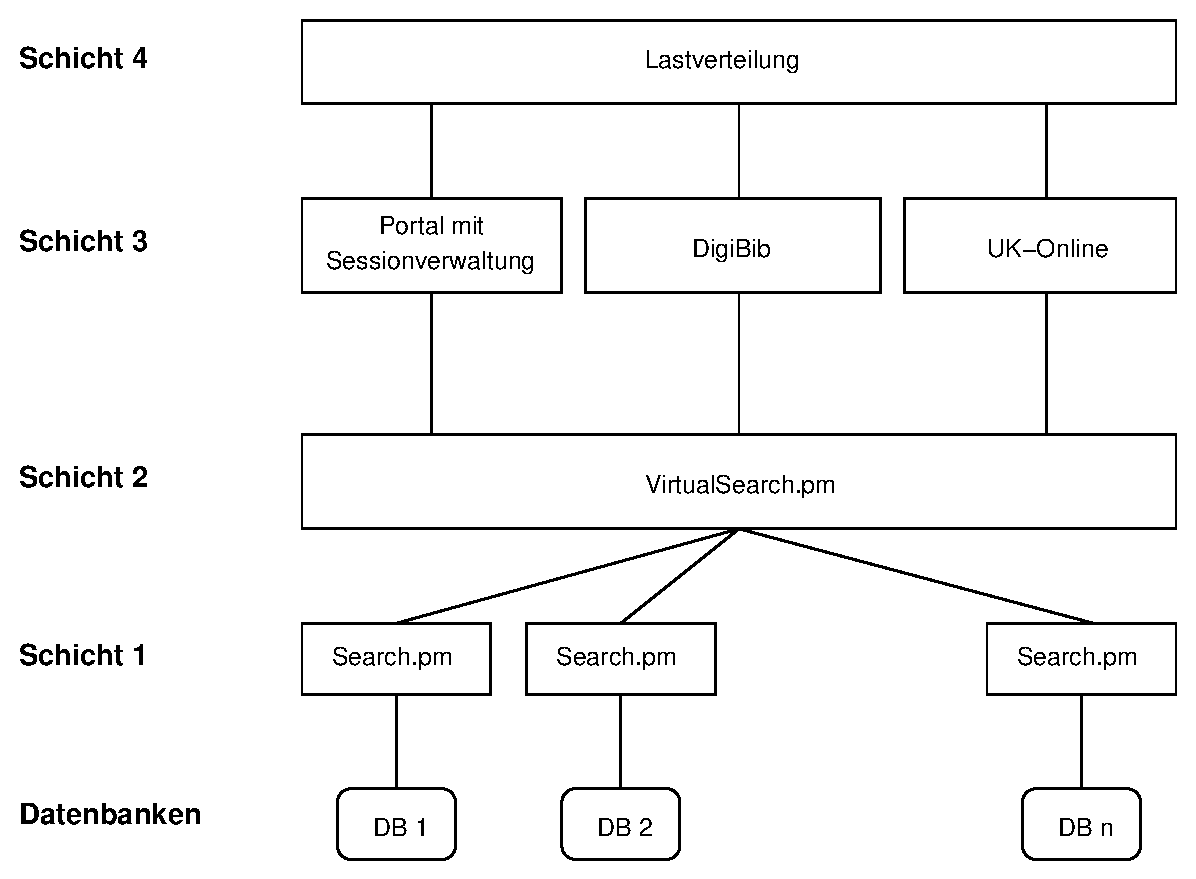
\includegraphics[width=12cm]{schicht04.eps}
    \end{minipage}
    \caption{Generelle Architektur der OpenBib-Portal-Suite}
  \label{bild:architektur}
  \vspace{3mm}
\end{shadowenv}
\end{figure}

\section{Die datenbankabhängige Schicht 1 -- \texttt{OpenBib::Search}}

In der untersten, der datenbankabhängigen Schicht greift das
Perl-Modul \texttt{OpenBib::Search} auf eine feste Datenbank zu.
Welche Datenbank dies ist, kann als Aufrufparamter dem Programm
mitgegeben werden. Dadurch ist es möglich, das gleiche Programm für
Recherchen über ver\-schie\-de\-ne Daten\-banken zu nutzen. Das Modul
selbst -- wie auch alle anderen unter
\begin{verbatim}
openbib/portal/perl/modules
\end{verbatim}
angesiedelten Module -- ist als Erweiterung des Apache-Webservers via
\texttt{mod\_perl} realisiert.  Dadurch arbeitet es außer\-ordentlich
schnell.


\section{Die datenbankübergreifende Recherche-Schicht 2 -- \texttt{OpenBib::VirtualSearch}}

Die datenbankübergreifende Recherche geschieht in der über
\texttt{OpenBib::Search} liegenden Schicht 2 (vgl. Abb.
\ref{bild:architektur}) mit dem Perl-Modul
\texttt{OpenBib::VirtualSearch}. Aufgabe dieses Modules ist es, eine
Suchanfrage und eine Anzahl an Recherche-Datenbanken vom Benutzer
entgegen\-zuneh\-men und genau diese eine Suchanfrage sequentiell an
jede der übergebenen Datenbanken zu schicken. Zu diesem Zweck werden
entsprechende Utility-Routinen aus dem im
\texttt{OpenBib::Search}-Kontext angesiedelten Modul
\texttt{OpenBib::Search::Util} verwendet.

Die Ergebnisse der einzelnen Recherchen werden entgegengenommen und in
Listenform auf\-be\-rei\-tet. Die jeweiligen Titel selbst sind in dieser
Gesamttrefferliste via URL mit einer Suchanfrage für genau diesen
Einzeltreffer mit \texttt{OpenBib::Search} verknüpft. 
Bei der
Auswahl eines einzelnen Treffers wird dadurch direkt in die
zugehörige Datenbank via \texttt{OpenBib::Search} gesprungen. 

Alle 'normalen' Verknüpfungs-Links (Normdaten, Hierarchien, etc.)
beziehen sich -- wir befinden uns nach der Auswahl eines Treffer wieder in
Schicht 1 -- auf genau diese eine Datenbank. Über das große
stilisierte 'G' bei den Normdaten kann jedoch auch an dieser Stelle
wieder eine datenbankübergreifende Recherche nach genau dem
zugehörigen Begriff gestartet werden. Der Benutzer hat somit bei
einem Einzeltreffer immer die Möglichkeit selbst zu entscheiden, ob
er sich bzgl. der Normdaten weiter im zugehörigen Katalog aufhalten
möchte, oder katalogübergreifend Recherchieren möchte.

Da in jedem Katalog die Verknüpfungen bereits in der Datenbank
existieren, ist ein 'sich treiben lassen' in einem festen Katalog
außer\-ordentlich schnell, während bei einer katalogübergreifenden
Suche ein kleiner Tribut zu zahlen ist, da nun effektiv wieder alle
Datenbanken mit einer 'neuen Suche' abgefragt werden.

Da \texttt{OpenBib::VirtualSearch} letztlich für die
datenbankübergreifende Gewinnung der Recherche\-er\-geb\-nisse
zuständig ist, werden nach erfolgreicher Recherche die Ergebnisse
aufgeteilt nach den einzelnen Katalogen in der Session-Datenbank
\texttt{session} 'gecached'. Durch das Caching der
Re\-cher\-che\-ergebnisse kann im Kontext von der Portal-Schicht 3
üeber das dort angesiedelte Modul \texttt{OpenBib::ResultLists} auch
eine Trefferlistenfunktionalität geleistet werden, in der man über
die Ergebnisse der letzten Recherche hinaus auch noch direkt auf die
Ergebnisse jeder zuvor eingegebenen Suche in der aktuellen Session
zugreifen kann.

\section{Die Portal-Schicht 3 mit weiteren externen Zugriffmechanismen}

\subsection{Das Portal mit Session- und Benutzerverwaltung}

In der Portalschicht wird dem Benutzer sessionbasiert in einer aus
zwei Frames bestehenden Web-Seite eine Arbeits- und Recherche-Oberfläche
geliefert. 

Der Einsprung-URL in das Portal wird durch das Modul
\texttt{OpenBib::StartOpac} realisiert.

Das Modul \texttt{OpenBib::StartOpac} kann über verschiedene
Parameter gesteuert werden, die z.B. für den direkten Sprung zu einem
einzelnen Treffer einer Datenbank oder der Anzeige einer
katalogeigenen Sicht des Portals Verwendung finden und gegebenenfalls
an nachgelagerte Module durchgereicht werden. Seine wesentliche
Aufgabe ist jedoch, eine eindeutige Session-ID zu generieren sowie ein
Frameset mit zwei Frames bereitzustellen.  Das obere Frame für die
Navigation wird durch das Modul \texttt{OpenBib::HeaderFrame}
gefüllt, das untere Frame standardmäßig zuerst durch das Modul
\texttt{OpenBib::SearchFrame}, das dem Navigations-Element 'Einfache
Recherche' bzw. 'Komplexe Recherche' entspricht.

Das Modul \texttt{OpenBib::HeaderFrame} ist für die Navigation im Portal
inklusive Counter für die Merkliste zuständig.

In der Navigation werden folgende Funktionalitäten angeboten:

\begin{description}
\item[Katalogauswahl] Die Auswahl der zu durchsuchenden Kataloge geschieht
  über eine entsprechende Aus\-wahl\-seite, die durch das Modul
  \texttt{OpenBib::DatabaseChoice} generiert wird.
\item[Recherche] Die Recherche-Maske wird über einen Aufruf von
  \texttt{OpenBib::SearchFrame} dargestellt.
\item[Trefferliste] Ein Zugriff auf Trefferlisten aus vorangegangenen
  Recherchen geschieht über das Modul \texttt{OpenBib::ResultLists},
  welches neben der verteilten Recherche auch für ein Caching der
  Ergebnis-Daten zuständig ist.
\item[Merkliste] Die Anzeige, Organisation sowie der Mailversand der
  Merkliste wird durch die Module
  \texttt{OpenBib::ManageCollection} und \texttt{OpenBib::MailCollection}
  über\-nom\-men. Bei Auswahl eines Treffers für die Merkliste wird
  \texttt{OpenBib::HeaderFrame} aktualisiert, und zeigt die neue Zahl
  gemerkter Treffer an.
\item[RSS] Über das Modul \texttt{OpenBib::RSSFrame} wird eine zu
  diesem View zugeordnete Liste an RSS-Feeds für die letzten 50
  Neuaufnahmen der entsprechenden Kataloge ausgegeben.
\item[Mein OpenBib] Über das Modul \texttt{OpenBib::Login}
  kann sich der Benutzer am Portal authentifizieren und so von
  weiteren personalisierten Funktionalitäten profitieren. Dazu
  gehören neben generellen Benutzereinstellungen
  (\texttt{OpenBib::UserPrefs}) u.a. per\-sis\-ten\-te Merklisten sowie
  Datenbankprofile (\texttt{OpenBib::DatabaseProfile}).

  Das Modul gewährt dabei den Zugang auf Grundlage seiner eigenen
  Datenbank, die über das Modul \texttt{OpenBib::SelfReg} via
  Selbstregistierung gefüllt wird, bzw. auf Grundlage von lokalen
  Bibliothekssystemen -- hier wird konkret das Bibliothekssystem Sisis
  SunRise unterstützt --, die über eine selbst entwicklte
  WebServices-Schnittstelle OLWS (Open Library WebServices)
  angesprochen werden können. Falls ein Benutzer sein
  selbstregistriertes Passwort vergessen hat, so kann er es sich über
  das Modul \texttt{OpenBib::MailPassword} per Mail zusenden lassen.
\item[Hilfe] Die Hilfeseite wird direkt als URL
  \texttt{/suchhilfe.html} angesprochen.
\item[Sitzung beenden] Beim Ende der Sitzung wird zum Modul
  \texttt{OpenBib::Leave} gesprungen, welches die sessionrelevanten Daten
  entfernt sowie einen URL in die Schicht 4 zur Lastver\-teilungs\-instanz
  \texttt{OpenBib::LoadBalancer} mit Angabe eines eventuell aktiven Views
  (Institutssicht) für einen er\-neu\-ten Einstieg in das Such-Portal
  bereitstellt.

\end{description}

\subsection{Externe Anbindung an die DigiBib}

Neben der Bereitstellung einer Recherche- und Arbeitsoberfläche für
den Endbenutzer, besteht auch die Möglichkeit über eine externe
Zugriffs-Schnittstelle automatisiert auf den Gesamtkatalog
zuzugreifen.

Eine solche Möglichkeit besteht in der Einbindung in das Such-Portal
\textbf{Digitale Bibliothek NRW} (DigiBib) des
Hoch\-schul\-bibliotheks\-zentrum NRW (hbz). Das Suchinterface besteht aus
einem fest definierten Such-URL und einem fest definierten
HTML-basierten Antwortformat für die Treffer. Grundsätzlich wird auf
eine Rechercheanfrage, z.B. unter Angabe eines Suchbegriffes für den
Titel, mit einer Kurztitelliste geantwortet. Es kann bestimmt werden,
welcher Teil der Kurztitelliste von den OpenBib-Daten\-banken
angefordert werden darf (Blätterfunktion mit frei wählbarem Offset
und Schrittweite). Darüber hinaus wird neben der Kurztitelliste auch
die Anzeige eines Einzeltreffers mit weiter\-gehen\-den Kategorien
angeboten. In der Kurztitelliste sind alle Informationen vorhanden, um
den Einzeltreffer aufzurufen.

\subsection{Externe Anbindung an UK-Online}

Eine weitere Anbindung besteht in das Universitätsportal UK-Online
von Herrn Prof. Lohnstein aus der Philosophischen Fakultät der
Universität zu Köln. Hier wird in UK-Online die Möglichkeit
angeboten eigenen Bibliographie-Listen zu verwalten. Der Aufbau einer
solchen Bibliographie-Liste geschieht über die Recherche in OpenBib
und anschließende Umwandlung und Ab\-spei\-cherung in ein
Bibliographie-Listen-Format.

Nach dem derzeitigen Stand sind beide externen Anbindung noch nicht in
einer lastverteilten Variante verfügbar. Diese ist jedoch kurz vor
der Fertigstellung.

\section{Die Lastverteilungs-Schicht 4}

Die Lastverteilungs-Schicht ist der erste Anlaufpunkt für die
Benutzung von OpenBib. Diese Schicht wird für das Portal durch das
Modul \texttt{OpenBib::LoadBalancer} und \texttt{OpenBib::ServerLoad} gebildet.
Entscheidungsgrundlage für die Verteilung ist die Auslastung der
betroffenen Recher, deren generelle Ansprechbarkeit sowie die
generelle Funktionsfähigkeit des MySQL-Daten\-bank\-sys\-tems.

Durch diese vorgeschaltete Verteilung der Recherche-Sitzungen auf
mehrere Rechner ergeben sich mehrere Vorteile:

\begin{enumerate}
\item Es wird eine Lastverteilung durchgeführt. Wenn also ein Nutzer
  einen dieser URL's aufruft, so wird er auf den Rechner
  weitergeleitet, der am wenigsten belastet ist.  Dies ist primärer
  Zweck dieser Schicht.
\item Ist ein Rechner defekt -- im Sinne von 'nicht ansprechbar'
  bzw. 'DBMS-seitig nicht funk\-tions\-fä\-hig' --, dann wird er bei der
  Verteilung/Weiterleitung nicht mehr berücksichtigt und die Benutzer
  werden nur noch auf die verbliebenen Rechner verteilt. In diesem
  Fall ist bei der Weiterleitung mit einer kurzen Wartezeit von
  maximal 5 Sekunden (Timeout) zu rechnen.  Automatisch wird
  zusätzlich an den Administrator eine Mail ge\-ne\-riert, die ihn
  auf den defekten Rechner hinweist. Ein Sonderfall ist natuerlich der
  'Verteilungs\-rech\-ner' selbst, bei dessen Ableben temporär ein
  anderer Rechner unter seiner Identität einspringen muß. Letzteres
  kann selbstverständlich nicht automatisch geschehen und muss
  manuell konfiguriert werden. In diesem Sinn besteht mit dem
  Lastverteilungsrechner ein Singe-Point-Of-Failure, der nur über
  HA-Mechanismen ausgeräumt werden kann.
\item Werden Wartungsarbeiten auf einem der Rechner ausgeführt, so
  kann man ihn selbst temporär aus der Verteilung/Weiterleitung
  herausnehmen. Auf diese Weise ändert sich für die Nutzer nichts,
  es werden dann die verbliebenen Rechner verwendet.
\end{enumerate}


\chapter{Konzepte und Interna von OpenBib}


\section{Kategorienformat}

Die bibliographische Datenhaltung in der MySQL-Datenbank ist
grundsätzlich unabhängig vom verwendeten Kategorienschema. Damit
können dort -- ohne Änderung oder Erweiterung der Datenbank --
beliebige andere Kategorien, als die aus dem an den MAB2-Standard angelehnte
Standardkategorien\-schema, abgelegt und verarbeitet werden.

Eine Kategorie in der bibliographischen Datenbank zeichnet sich durch
folgendes aus:

\begin{itemize}
\item Eine Kategorie gehört zu einem Normdatentyp. Mögliche
  Normdatentypen sind Titel (tit, \textbf{T}, \texttt{1}), Verfasser
  bzw. Person (aut, \textbf{P}, \texttt{2}), Körperschaft bzw. Urheber
  (kor, \textbf{C}, \texttt{3}), Schlagworte (swt, \textbf{S},
  \texttt{4}), Systematik bzw. Notation (notaton, \textbf{N},
  \texttt{5}) und Exemplare (mex, \textbf{X}, \texttt{6}).
\item Eine Kategorie besteht aus der numerischen Id bezogen auf einen
  Normdatentyp, einer Kategorienummer, einem numerischen
  Indikator\footnote{Mit dem numerischen Indikator können entweder
    alphabetische Indikatoren gemappt werden (a gleich 1, b gleich 2
    usw.), eine Multiplizität der Kategorie ausgedrückt werden (1.
    Exemplar gleich 1, 2. Exemplar gleich 2) oder auch beides zusammen
    über Modulos (a des 1. Exemplars gleich 1, b des 1. Exemplars
    gleich 2, a des 2. Exemplars gleich 3, b des 2. Exemplars gleich
    4)}.
\item Jeder Kategorie ist ein abstrakter Bezeichner zugeordnet, dem
  wiederum pro Sprache ein Beschreibungstext zugeordnet werden
  kann. Pro Datenbank können bei Bedarf andere Beschreibungstexte
  zugeordnet werden
\end{itemize}


\subsection{Beispiel}

Als Beispiel verwenden wir die Titelaufnahme des Hauptaufnahme des
mehrbändigen Werkes \emph{TCP/IP Illustrated} von \emph{Richard
  W. Stevens}. Diese Titelaufnahme sieht wie folgt aus:

\begin{shadowenv}
\vspace{0.5cm}
\begin{center}
  \begin{tabular}{ll}
id	        & 5899\\
Verfasser	& Stevens, W. R.\\
HST	        & TCP/IP Illustrated\\
Vorl.Verfasser	& W. Richard Stevens\\
Verlagsort	& Reading, Mass. [u.a.]\\
Verlag	        & Addison-Wesley\\
Schlagwort	& TCP / IP\\
Schlagwort	& Internet\\
Schlagwort	& Kommunikationsprotokoll\\
Unterordnungen	& 2\\
  \end{tabular}
\end{center}
  \caption{Beispiel-Titel}
\vspace{0.5cm}
\end{shadowenv}


\subsubsection{Verknüpfungen}
Dieser Titel verteilt sich nun mit seinen Daten auf mehrere
Normdaten-Tabellen. Es sind dies hier konkret die Titeltabelle
\texttt{tit}, die Verfassertabelle \texttt{aut}, die Schlagworttabelle
\texttt{swt} sowie für die Verknüpfungen des Titelsatzes mit den
anderen Normdaten und die Abhängigkeiten zwischen Titeln
(Unterordnungen) die Verknüpfungstabelle \texttt{conn}.

Zunächst werden für diesen Titel die Informationen in der
Titelnormdaten-Tabelle dargestellt mit 

\begin{verbatim}
mysql> select * from tit where id=5899;
\end{verbatim}

dargestellt.

\begin{verbatim}
+------+----------+-----------+-----------------------+
| id   | category | indicator | content               |
+------+----------+-----------+-----------------------+
| 5899 |        1 |         0 | 05899                 |
| 5899 |        2 |         0 | 27.05.2003            |
| 5899 |      331 |         1 | TCP/IP Illustrated    |
| 5899 |      359 |         1 | W. Richard Stevens    |
| 5899 |      410 |         1 | Reading, Mass. [u.a.] |
| 5899 |      412 |         1 | Addison-Wesley        |
+------+----------+-----------+-----------------------+
6 rows in set (0.30 sec)
\end{verbatim}


Dieser Titelsatz ist mit den anderen Normdaten verknüpft. Die Ids der
verknüpften Sätze erhält man mit

\begin{verbatim}
mysql> select * from conn where    (sourceid=5899 and sourcetype=1) 
                                or (targetid=5899 and targettype=1);
\end{verbatim}

zu:

\begin{verbatim}
+----------+----------+------------+----------+------------+------------+
| category | sourceid | sourcetype | targetid | targettype | supplement |
+----------+----------+------------+----------+------------+------------+
|      100 |     5899 |          1 |      684 |          2 |            |
|      710 |     5899 |          1 |      133 |          4 |            |
|      710 |     5899 |          1 |      604 |          4 |            |
|      710 |     5899 |          1 |      571 |          4 |            |
|        0 |     5900 |          1 |     5899 |          1 |            |
|        0 |     5901 |          1 |     5899 |          1 |            |
+----------+----------+------------+----------+------------+------------+
6 rows in set (0.11 sec)
\end{verbatim}

Es ist damit ersichtlich, dass 

\begin{itemize}
\item der Verfasser des Titels (\texttt{category:100}, \texttt{targettype:2}) die Id \texttt{684} hat
\item die drei Schlagworte des Titels (\texttt{category:710)}) die Ids
  \texttt{133}, \texttt{604} sowie \texttt{571} haben
\item Die Unterordnungen des Titels (\texttt{sourceid}) die Titel-Id's
  \texttt{5900} und \texttt{5901} haben.
\end{itemize}

Damit ergibt sich der Verfasser mit

\begin{verbatim}
mysql> select * from aut where id=684;
\end{verbatim}

zu 

\begin{verbatim}
+-----+----------+-----------+---------------------+
| id  | category | indicator | content             |
+-----+----------+-----------+---------------------+
| 684 |        1 |         0 | Stevens, W. R.      |
| 684 |      102 |         1 | Stevens, W. Richard |
+-----+----------+-----------+---------------------+
2 rows in set (0.04 sec)
\end{verbatim}

sowie die Schlagworte mit 

\begin{verbatim}
mysql> select * from swt where id in (133,604,571);
\end{verbatim}
zu

\begin{verbatim}
+-----+----------+-----------+--------------------------------------------------+
| id  | category | indicator | content                                          |
+-----+----------+-----------+--------------------------------------------------+
| 133 |        1 |         1 | TCP / IP                                         |
| 133 |      113 |         1 | Kommunikationsprotokoll                          |
| 133 |      108 |         1 | 30m                                              |
| 133 |      102 |         1 | Transmission control protocol / Internet protocol|

| 571 |        1 |         1 | Kommunikationsprotokoll                          |
| 571 |      108 |         1 | 30                                               |
| 571 |      102 |         3 | Kommunikationstechnik                            |
| 571 |      102 |         2 | Datenübertragung                                 |
| 571 |      102 |         1 | Übertragungsprotokoll                            |

| 604 |        1 |         1 | Internet                                         |
| 604 |      108 |         1 | 30m                                              |
| 604 |      102 |         2 | TCP / IP / Internetzwerk                         |
| 604 |      102 |         1 | Internetzwerk / TCP / IP                         |
+-----+----------+-----------+--------------------------------------------------+
\end{verbatim}

Für die untergeordneten Titel wiederholt sich diese gesamt Prozedur
mit den zweit Titel-ID's \texttt{5900} und \texttt{5901}.

\subsubsection{Internationalisierung}

Für die Internationalisierung der Bezeichnungstexte wird für die
einzelnen Titelkategorien ein Bezeichner durch Vornullen der
Kategorienummer auf 4 stellen sowie Voranstellen des Normdatenkürzels.

Damit erhält man für den Titel folgende Bezeichner

\begin{description}
\item[T0100] Aus der Kategorie \texttt{100} von \texttt{conn}
\item[T0331] Aus der Kategorie \texttt{331} von \texttt{tit}
\item[T0359] Aus der Kategorie \texttt{359} von \texttt{tit}
\item[T0410] Aus der Kategorie \texttt{410} von \texttt{tit}
\item[T0412] Aus der Kategorie \texttt{412} von \texttt{tit}
\item[T0710] Aus der Kategorie \texttt{710} von \texttt{conn}
\item[T5000] Aus der Anzahl der Verweise in \texttt{conn}.
\end{description}

\appendix

\chapter{Tabellen in \texttt{session.mysql}}

In diesem Anhang werden die einzelnen Tabellen in der
Session-Datenbank beschrieben.

Diese Tabellen verteilen sich auf rein session-basierte Aufgaben sowie
allgemeine Konfigurations\-ein\-stellungen des Portals.


\section{Tabellen zu session-basierten Aufgaben}

\begin{description}
\item[session] Dies ist die primäre Tabelle in der die
  \texttt{sessionid} für eine Nutzersitzung abgespeichert wird.
  Zusätzlich werden folgende Informationen gespeichert:
  \begin{description}
  \item[createtime] Anfangszeit der Session.
  \item[lastresultset] Geordnete Liste der Katalog-ID's zur letzten
    Rechercheanfrage. Mit dieser Liste wird die katalogübergreifende
    Titelnavigation in der Einzeltrefferanzeige realisiert.
  \item[queryoptions] Allgemeine Suchoptionen. Durch die zentrale Speicherung der
    Suchoptionen brauchen diese nicht bei den internen URL-Verweisen
    verwendet werden.
  \end{description}
die Anfangszeit der Session \texttt{createtime}
  gespeichert. 
\item[treffer] Diese Tabelle realisiert sessionabhängig die
  \textbf{Merkliste}. Es werden zu jeder Session der Datenbankname sowie die
  Identifikations-Nr des gemerkten Titels abgespeichert. Anhand dieser
  Informationen wird die Merkliste bei ihrem Aufruf sekundenaktuell
  mit dem etwaig vorhandenen Ausleihstatus der entsprechenden
  Titelsätze aufgebaut.
\item[sessionlog] Diese Tabelle soll im Betrieb mit relevanten
  Informationen gefüllt werden, die dann statistisch ausgewertet
  werden können. Derzeit wird sie nicht verwendet.
\item[queries] In dieser Tabelle werden sessionabhängig die
  Suchanfragen inkl. gefundener Treffer ab\-ge\-spei\-chert. Dadurch ist es
  möglich, sich ältere Suchanfragen wieder in die Recherchemaske
  eintragen zu lassen.
\item[dbchoice] In dieser Tabelle wird die vom Benutzer vorgenommene
  Datenbankauswahl session\-ab\-hängig abgespeichert.
\item[searchresults] In dieser Tabelle wird session\-ab\-hän\-gig zu jeder
  Suchanfrage (\texttt{queryid} der \texttt{queries}-Tabelle) pro
  Datenbank das Ergebnis gecached. Zusätzlich wird jeweils auch noch
  die Anzahl der Treffer in der jeweiligen Datenbank
  ab\-ge\-spei\-chert. Durch diese Tabelle in Verbindung mit der Tabelle
  \texttt{queries} wird die \textbf{Trefferliste} realisiert.
\item[sessionview] Über diese Tabelle wird die Nutzung eines Views
  durch eine Session festgehalten. Diese Information wird benötigt,
  damit im oberen Frame (\texttt{OpenBib::HeaderFrame}) wie auch in der
  Recherchemaske (\texttt{OpenBib::SearchFrame}) die View-Informationen
  zusätzlich angezeigt werden. Derzeit wird in \texttt{OpenBib::HeaderFrame}
  auf ein Bild mit dem Namen des Views
\begin{verbatim}
HTDOCS/images/openbib/views/<viewname>.png
\end{verbatim}

  verwiesen.
\item[sessionmask] In dieser Tabelle wird festgehalten, welche
  Recherchemaske -- Einfache Recherche oder Komplexe Recherche -- der
  Nutzer zuletzt aktiviert hat. Bei einer Aktivierung des allgemeinen
  Ober-Menueintrags 'Recherche' wird dann diese konkrete
  Recherchemaske aus\-ge\-ge\-ben.
\item[sessionprofile] \dots
\end{description}

\section{Tabellen zu allgemeinen Konfigurationseinstellungen des Portals}

\begin{description}
\item[dbinfo] In dieser Tabelle werden Informationen zu den einzelnen
  Katalogdatenbanken ab\-ge\-spei\-chert. Dazu gehört die Fakultät
  (\texttt{faculty}, derzeit fest in den Modulen einprogrammiert),
  eine Beschreibung (\texttt{description}), das Katalogisierungssystem
  (\texttt{system} anhand Kürzel), der Datenbankname
  (\texttt{dbname}), das Bibliothekssigel (\texttt{sigel}) und
  schließlich die wesentliche Information, ob die Daten\-bank im Portal
  aktiv ist oder nicht (\texttt{active}). Über die letzte Einstellung
  lassen sich im laufenden Betrieb Daten\-banken ein- und ausblenden.
\item[dboptions] Zu jeder Daten\-bank werden hier Informationen
  abgelegt, wo die zum Aufbau der Daten\-bank notwendigen Daten liegen
  und alle zum Heranschaffen der Daten benötigten Informationen wie
  Rechnername (\texttt{host}), Pfade, Dateinamen, Zugriffsprotokoll
  (\texttt{lokal}, \texttt{http}, \texttt{ftp}) und
  Authentifizierungsinformationen wie Benutzernamen oder Passworte.
  Derzeit sind diese Informationen schon im Wesentlichen vorhanden,
  sie werden durch die automatischen Konvertierungsskripte jedoch noch
  nicht verwendet.
\item[titcount] In dieser Tabelle wird die Anzahl der Titel pro
  Daten\-bank festgehalten. Diese Information wird über das Modul
  \texttt{OpenBib::SearchFrame} für den Benutzer ausgegeben. Das Setzen
  dieser Werte geschieht über die automatischen
  Konvertierungsskripte.
\item[rssfeeds] In dieser Tabelle werden alle verfuegbaren Typen an RSS-Feeds
  zu den einzelnen Daten\-bank aus \texttt{dbinfo} definiert. Die
  RSS-Feeds lassen sich hier nach deren Konfiguration generell
  aktivieren sowie deaktivieren.
\item[rsscache] Um die Antwortzeiten bei der Generierung eines
  RSS-Feeds zu minimieren, wird ein RSS-Cache mit einer
  Aktivitätsdauer von 12 Stunden verwendet.
\item[viewinfo] In dieser Tabelle werden zu einer Recherche-Sicht
  (view) neben dem den View de\-fi\-nier\-enden Viewnamen
  (\texttt{viewname}) auch eine Beschreibung \texttt{description}
  abgelegt. Die Informatione, ob der View aktiv ist oder nicht
  (\texttt{active}) wird derzeit nicht genutzt.
\item[viewdbs] In dieser Tabelle werden zu dem Viewnamen die Daten\-banken
  festgelegt, die mit der konkreten Recherche-Sicht assoziiert
  sind. Hier können auch mehrere Daten\-banken ein\-ge\-tra\-gen werden.
\item[viewrssfeeds] In dieser Tabellen werden zu einem View die
  RSS-Feeds konfiguriert, die in diesem View über den Menu-Punkt
  \texttt{RSS} angezeigt werden sollen

\end{description}



\chapter{Tabellen in \texttt{pool.mysql}}

Die Tabellen in \texttt{pool.mysql} werden nach Norm- bzw.
Stamm-Dateien geordnet dargestellt. Es sind dies \emph{Titel},
\emph{Verfasser}, \emph{Körperschaften}, \emph{Notationen},
\emph{Schlagworte} sowie \emph{Exemplardaten}. Darüber hinaus gibt es eine zusätzliche
Tabelle \texttt{search} in der in Form einer Volltextsuche
recherchiert werden kann. Verknüpfungen zwischen den Norm-Dateien
werden über die Tabelle \texttt{conn} abgebildet.

\section{Titel-Normdaten}

\begin{description}
\item[tit] In dieser Tabelle befinden sich die für die Anzeige
  bestimmten Titeldaten. Grundsätzlich werden in dieser Tabelle
  folgende Informationen in einem Metadaten-unabhängigen Format
  abgelegt.
  \begin{description}
  \item[id] Identifikationsnummer
  \item[category] Kategoriename -- sie basiert auf auf MAB2-Kategorienummer
  \item[indicator] Indikator -- transformiert von alphabetisch nach numerisch
  \item[content] Eigentlicher Kategorieinhalt
  \end{description}
\item[tit\_ft] Kategorien, die über einen Volltextindex recherchierbar
  gemacht werden.
  \begin{description}
  \item[id] Identifikationsnummer
  \item[category] Kategoriename -- sie basiert auf auf MAB2-Kategorienummer
  \item[content] Eigentlicher Kategorieinhalt, der suchbar gemacht wird.
  \end{description}
\item[tit\_string] Kategorien, die über eine Wortanfangssuche
  recherchierbar gemacht werden.
  \begin{description}
  \item[id] Identifikationsnummer
  \item[category] Kategoriename -- sie basiert auf auf MAB2-Kategorienummer
  \item[content] Eigentlicher Kategorieinhalt, der suchbar gemacht wird.
  \end{description}
\end{description}

\section{Verfasser-Normdaten}

\begin{description}
\item[aut] In dieser Tabelle befinden sich die für die Anzeige
  bestimmten Verfasserinformationen für die Kategorien
  \textbf{Verfasser} und \textbf{Person}. Grundsätzlich werden in
  dieser Tabelle folgende Informationen in einem
  Metadaten-unabhängigen Format abgelegt.
  \begin{description}
  \item[id] Identifikationsnummer
  \item[category] Kategoriename -- eigentlich eine interne Kategorienummer
  \item[indicator] Indikator -- transformiert von alphabetisch nach numerisch
  \item[content] Eigentlicher Kategorieinhalt
  \end{description}
\item[aut\_ft] Kategorien, die über einen Volltextindex recherchierbar
  gemacht werden.
  \begin{description}
  \item[id] Identifikationsnummer
  \item[category] Kategoriename -- eigentlich eine interne Kategorienummer
  \item[content] Eigentlicher Kategorieinhalt, der suchbar gemacht wird.
  \end{description}
\item[aut\_string] Kategorien, die über eine Wortanfangssuche
  recherchierbar gemacht werden.
  \begin{description}
  \item[id] Identifikationsnummer
  \item[category] Kategoriename -- eigentlich eine interne Kategorienummer
  \item[content] Eigentlicher Kategorieinhalt, der suchbar gemacht wird.
  \end{description}
\end{description}

\section{Körperschafts-Normdaten}

\begin{description}
\item[kor] In dieser Tabelle befinden sich die für die Anzeige
  bestimmten Körperschaftsinformationen für die Kategorien
  \textbf{Körperschaft} und \textbf{Urheber}. Grundsätzlich werden in
  dieser Tabelle folgende Informationen in einem
  Metadaten-unabhängigen Format abgelegt.
  \begin{description}
  \item[id] Identifikationsnummer
  \item[category] Kategoriename -- eigentlich eine interne Kategorienummer
  \item[indicator] Indikator -- transformiert von alphabetisch nach numerisch
  \item[content] Eigentlicher Kategorieinhalt
  \end{description}
\item[kor\_ft] Kategorien, die über einen Volltextindex recherchierbar
  gemacht werden.
  \begin{description}
  \item[id] Identifikationsnummer
  \item[category] Kategoriename -- eigentlich eine interne Kategorienummer
  \item[content] Eigentlicher Kategorieinhalt, der suchbar gemacht wird.
  \end{description}
\item[kor\_string] Kategorien, die über eine Wortanfangssuche
  recherchierbar gemacht werden.
  \begin{description}
  \item[id] Identifikationsnummer
  \item[category] Kategoriename -- eigentlich eine interne Kategorienummer
  \item[content] Eigentlicher Kategorieinhalt, der suchbar gemacht wird.
  \end{description}
\end{description}

\section{Schlagwort-Normdaten}

\begin{description}
\item[swt] In dieser Tabelle befinden sich die für die Anzeige
  bestimmten Körperschaftsinformationen für die Kategorie
  \textbf{Schlagwort}. Grundsätzlich werden in dieser Tabelle
  folgende Informationen in einem Metadaten-unabhängigen Format
  abgelegt.
  \begin{description}
  \item[id] Identifikationsnummer
  \item[category] Kategoriename -- eigentlich eine interne Kategorienummer
  \item[indicator] Indikator -- transformiert von alphabetisch nach numerisch
  \item[content] Eigentlicher Kategorieinhalt
  \end{description}
\item[swt\_ft] Kategorien, die über einen Volltextindex recherchierbar
  gemacht werden.
  \begin{description}
  \item[id] Identifikationsnummer
  \item[category] Kategoriename -- eigentlich eine interne Kategorienummer
  \item[content] Eigentlicher Kategorieinhalt, der suchbar gemacht wird.
  \end{description}
\item[swt\_string] Kategorien, die über eine Wortanfangssuche
  recherchierbar gemacht werden.
  \begin{description}
  \item[id] Identifikationsnummer
  \item[category] Kategoriename -- eigentlich eine interne Kategorienummer
  \item[content] Eigentlicher Kategorieinhalt, der suchbar gemacht wird.
  \end{description}
\end{description}

\section{Notations-Normdaten}

\begin{description}
\item[notation] In dieser Tabelle befinden sich die für die Anzeige
  bestimmten Notationsinformationen für die Kategorie
  \textbf{Notation}. Grundsätzlich werden in dieser Tabelle
  folgende Informationen in einem Metadaten-unabhängigen Format
  abgelegt.
  \begin{description}
  \item[id] Identifikationsnummer
  \item[category] Kategoriename -- eigentlich eine interne Kategorienummer
  \item[indicator] Indikator -- transformiert von alphabetisch nach numerisch
  \item[content] Eigentlicher Kategorieinhalt
  \end{description}
\item[notation\_ft] Kategorien, die über einen Volltextindex recherchierbar
  gemacht werden.
  \begin{description}
  \item[id] Identifikationsnummer
  \item[category] Kategoriename -- eigentlich eine interne Kategorienummer
  \item[content] Eigentlicher Kategorieinhalt, der suchbar gemacht wird.
  \end{description}
\item[notation\_string] Kategorien, die über eine Wortanfangssuche
  recherchierbar gemacht werden.
  \begin{description}
  \item[id] Identifikationsnummer
  \item[category] Kategoriename -- eigentlich eine interne Kategorienummer
  \item[content] Eigentlicher Kategorieinhalt, der suchbar gemacht wird.
  \end{description}
\end{description}

\section{Exemplar-Daten}

\begin{description}
\item[mex] In dieser Tabelle befinden sich die für die Anzeige
  bestimmten Exemplarinformationen aus dem Titeldatenbereich.
  Grundsätzlich werden in dieser Tabelle folgende Informationen in
  einem Metadaten-unabhängigen Format abgelegt.
  \begin{description}
  \item[id] Identifikationsnummer
  \item[category] Kategoriename -- eigentlich eine interne Kategorienummer
  \item[indicator] Indikator -- transformiert von alphabetisch nach numerisch
  \item[content] Eigentlicher Kategorieinhalt
  \end{description}
\item[mex\_ft] Kategorien, die über einen Volltextindex recherchierbar
  gemacht werden.
  \begin{description}
  \item[id] Identifikationsnummer
  \item[category] Kategoriename -- eigentlich eine interne Kategorienummer
  \item[content] Eigentlicher Kategorieinhalt, der suchbar gemacht wird.
  \end{description}
\item[mex\_string] Kategorien, die über eine Wortanfangssuche
  recherchierbar gemacht werden.
  \begin{description}
  \item[id] Identifikationsnummer
  \item[category] Kategoriename -- eigentlich eine interne Kategorienummer
  \item[content] Eigentlicher Kategorieinhalt, der suchbar gemacht wird.
  \end{description}
\end{description}

\section{Verknüpfungen zwischen den Normdaten}

\begin{description}
\item[conn] In dieser Tabelle befinden sich
  Verknüpfungsinformationen für die Normdaten. 
  Grundsätzlich werden in dieser Tabelle folgende Informationen in
  einem Metadaten-unabhängigen Format abgelegt.
  \begin{description}
  \item[category] Kategorie(nummer), der die Verknüpfung zugeordnet
    ist (z.B. Verfasser vs. Person)
  \item[sourceid] Id des zu verknüpfenden Satzes
  \item[sourcetype] Normdatei des zu verknüpfenden Satzes
  \item[targetid] Id des verknüpften Satzes
  \item[targettype] Normdatei des verknüpften Satzes
  \item[supplement] Zusatzinformation, die der Verknüpfung zugeordnet
    ist (z.B. [Hrsg.])
  \end{description}
\end{description}


\section{Recherche-Tabelle \texttt{search}}

Sämtliche vom Benutzer eingegebenen Suchbegriffe werden in der Tabelle
\texttt{search} recherchiert. Als Ergebnis der Suche werden
Identifikationsnummern (IDN's, Katkeys) der gefundenen Titel-Sätze
zurückgeliefert. Mit diesen IDN's wird dann in die Norm- bzw.
Stammdateien gesprungen, um alle Informationen zu diesen Titel-Sätzen
zu gewinnen. Diese Funktionalität wird allein von dem Modul
\texttt{OpenBib::Search} geleistet.

\chapter{Module geordnet nach Funktion bzw. Schicht}


\section{Schichtübergreifend}


\begin{itemize}
\item \texttt{OpenBib::Config}
\end{itemize}

\section{Schicht 1 - Zugriff auf Katalogdatenbank}

\begin{itemize}
\item \texttt{OpenBib::Search}
\end{itemize}

\section{Schicht 2 - Zugriff auf versch. Datenbanken der Schicht 1}

\begin{itemize}
\item \texttt{OpenBib::VirtualSearch}
\end{itemize}

\section{Schicht 3 - Rechercheportal}

\begin{itemize}
\item \texttt{OpenBib::DatabaseChoice}
\item \texttt{OpenBib::DatabaseProfile}
\item \texttt{OpenBib::HeaderFrame}
\item \texttt{OpenBib::Leave}
\item \texttt{OpenBib::Login}
\item \texttt{OpenBib::MailCollection}
\item \texttt{OpenBib::MailPassword}
\item \texttt{OpenBib::ManageCollection}
\item \texttt{OpenBib::SearchFrame}
\item \texttt{OpenBib::SelfReg}
\item \texttt{OpenBib::StartOpac}
\item \texttt{OpenBib::UserPrefs}
\end{itemize}

\section{Schicht 4 - Lastverteilung}

\begin{itemize}
\item \texttt{OpenBib::LoadBalancer}
\item \texttt{OpenBib::ServerLoad}
\end{itemize}


\begin{thebibliography}{ChBr82}
\originalTeX

\bibitem[FliHof06]{FlimmHoffJB:06} O.~Flimm, Chr. Hoffrath: \emph{Der
    Weg des KUG zum umfassenden Recherche-Portal}; erscheint in:
  Kooperative Informationsverarbeitung an der Universität zu Köln -
  Bericht für das Jahr 2005 (2006).
\bibitem[BoeFli:06]{BoeFli:EinbandDB} R.~Boeff, O.~Flimm: \emph{Von
    der traditionellen zur digitalen Sammlung historischer und
    künstlerischer Bucheinbände der USB Köln mit einem Einblick in die
    technische Konzeption der Datenbank}. -- in: Bibliothek. Forschung
  und Praxis. Jahrgang 30 (2006) Nr. 1, S.63
\end{thebibliography}
\germanTeX

\end{document}